% Appendix G

\chapter{Surface potential determination $\varphi_{s0}$ at zero gate voltage.}\label{app:AppendixG}
\lhead{Appendix G. \emph{Surface potential determination $\varphi_{s0}$ at zero gate voltage}}

In relation~\ref{eq:F.4}, the expression $\varphi_{s0}$ stands out,
which represents the surface potential of the MOS semiconductor
structure in the case of no external voltage is applied to the MOS
structure.  This potential is due to the difference in the output work
of the metal and the semiconductor and the charges located in the
insulator and at its interface with the semiconductor. At determine
this constant, we use a comparison of the measured and theoretical
dependence of $\varphi_{s}$ on the width of the OPN, as shown
v~\cite{App.3}. The OPN width for the experimental dependence
$\varphi_{s}(w)$ is determined from the relation

\begin{equation}\label{eq:G.1}
  w = \epsilon \bigg[\frac{1}{C_{mos}^{HF}} - \frac{1}{C_{ox}}\bigg]
\end{equation}

To determine the theoretical dependence of $\varphi_{s}(w)$ we use the
approximation described in~\cite{App.5}

\begin{equation}\label{eq:G.2}
  \beta \varphi_{s} = \frac{1}{2} {\bigg[\frac{w}{L_{DE}}\bigg]}^2 + \frac{1}{N_{B}L_{DE}}^{2} \int_{0}^{w}x[N(x)-N_{B}]dx + 1
\end{equation}

where $L_{DE}$ is the extrinsic Debay length, $N_{B}$ the
concentration of the substrate, and $N(x)$ the concentration of the
interfering impurities in subsurface region of the semiconductor. In
Figure~\ref{fig:App.3} is shown for the measured data of the Q-C
method from Figure~\ref{fig:3.4}. The value of $\varphi_{s0}$ is then
determined from the difference of the experimental and theoretical
dependence of $\varphi_{s}(w)$ at depth w, which corresponds to the
depletion state of the MOS structure. As shown v~\cite{App.3}
approximation~\ref{eq:G.2} ignores free charge carriers, which implies
its restriction of validity to the depletion state only.  The
integration constant can also be computed in the above manner when
calculating dependence of $\varphi_{s}(V_{g})$ using the Berglund
integral.

\begin{figure}[h!]\centering
  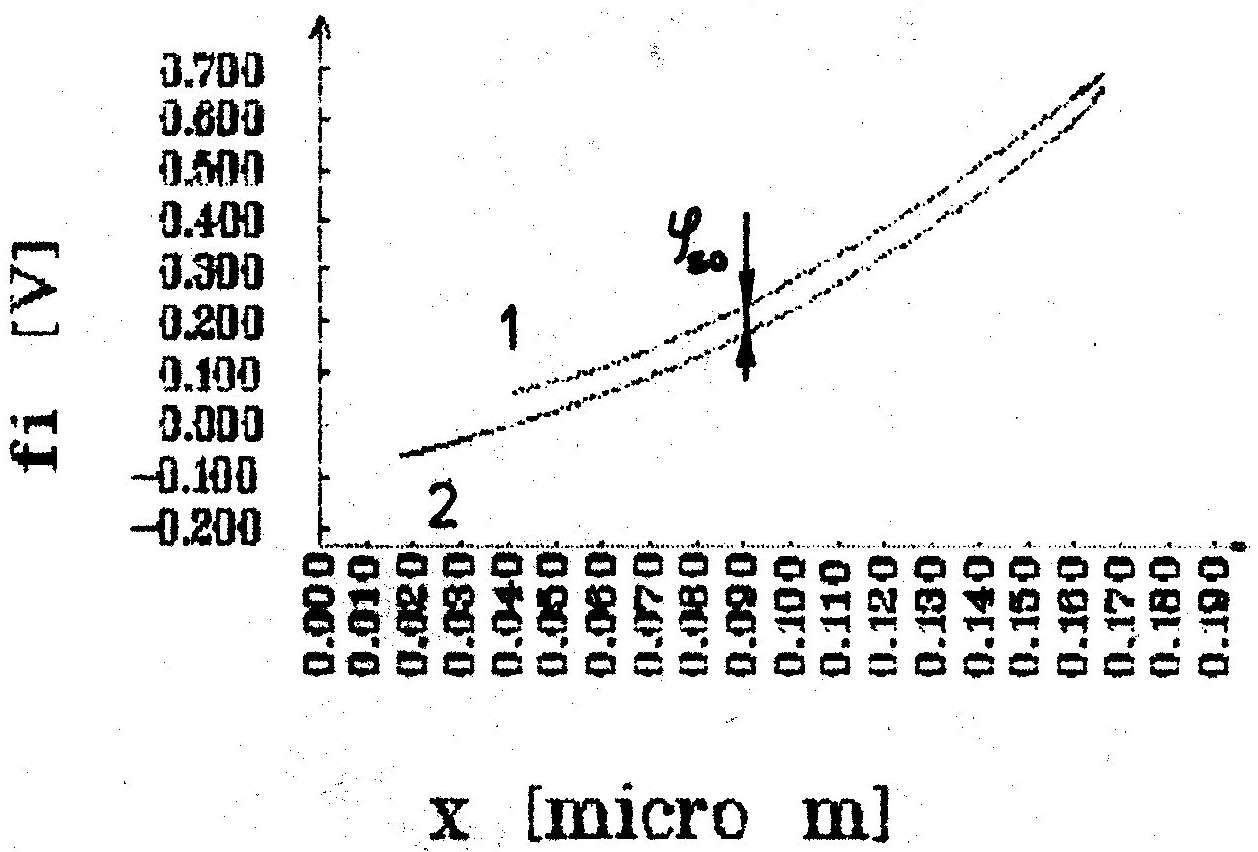
\includegraphics{Figures/fig-app-3.eps}
    \caption[Surface potential as a function of OPN width for MOS
      structure driven to a deep depletion state]{Process of surface
      potential as a function of OPN width for a MOS structure brought
      to the deep depletion state.  Curve 1 represents the
      $\varphi(x)$ waveform calculated from the relation~\ref{eq:G.2}
      and curve 2 shows the dependence determined from experimental
      data using relation~\ref{eq:F.4}.}\label{fig:App.3}
\end{figure}
% OBR10.BIT
